\chapter{Data and Methods}

\section{Data}
While examining both proposed methods for their suitability for near-infrared colorization, multiple datasets
and two data sources \textit{Caltech Camera Traps} \parencite{caltech} and \textit{Snapshot Serengeti} \parencite{serengeti} were used.

\subsection{Caltech Camera Traps}
\label{sec:cct}
\textit{Caltech Camera Traps} (CCT) is a dataset consisting of $243.100$ images from $140$ camera locations
in the southwestern United States with $21$ animal label categories \parencite{caltech}.
In particular, it primarily contains near-infrared images for the night and regular RGB images for images captured during the day.
Approximately $70 \%$ of the overall image set is labeled empty.
Annotations are provided in the \textit{COCO Camera Traps} format, describing meta information via JSON \parencite{caltech}
This allows an automatic parsing of the available images as well as efficient access to information about
the images, which comes in useful when creating sub-datasets for training networks.

\subsection{Snapshot Serengeti}
In contrast to the CCT dataset, \textit{Snapshot Serengeti} is a much larger dataset and comes from the Snapshot Serengeti National Park in Tanzania.
It consists of $7.1$ million images through seven seasons of the Snapshot Serengeti Project \parencite{serengeti}.
There are $61$ labeled species, where approximately $76\%$ of the images are labeled empty.
Similar to the CCT dataset, Snapshot Serengeti contains near-infrared images as well as RGB images and
is annotated in the COCO Camera Traps format \parencite{serengeti}. Therefore, dataset tooling can be used for both datasets.
Unlike the CCT dataset, Snapshot Serengeti employed multiple cameras for images captured at night.
Scoutgard's SG565 cameras produce RGB \textbf{night} images using an \textit{incandescent} flash and DLC Covert II cameras use an infrared flash and therefore produce NIR night images \parencite{serengeti}.

\subsection{Data Preprocessing}
\label{sec:subset-generation}
Since both datasets (CCT and Snapshot Serengeti) are substantially larger than processable for training, choosing a subset of these images is essential.
The requirements for this subset strongly influence the training performance of the translation models.

\begin{enumerate}
   \item Both network architectures require the dataset to be divided into an input domain (NIR) and an output domain (RGB). \label{item:requirement-split}
   \item To gain model performance in the main objective, which is to colorize the NIR images of \textit{animals}, it is important to choose only images that contain animals. \label{item:requirement-animal-filter}
   \item Training with a variety of image locations proves to decrease overfitting for the translation, and therefore a uniform distribution of the available locations should be approximated.
         Additionally, utilizing a random crop for each image can also help mitigate overfitting, and therefore, it is suggested. \label{item:requirement-weighted-sampling}
   \item Since most NIR images are taken at night, the network should not be influenced to solve the more difficult
         task of translating images from NIR night to RGB day. This can be achieved by only allowing night images for both
         domains. \label{item:requirement-night}
\end{enumerate}


The \ref{item:requirement-animal-filter}., \ref{item:requirement-weighted-sampling}. and \ref{item:requirement-night}. requirements are all achievable by using the information provided in the COCO format, and therefore,
are already obtainable before downloading a single image.
Only choosing images with animals \ref{item:requirement-animal-filter} is done by a simple filter on the data source before sampling.
The approximately uniform distribution of locations \ref{item:requirement-weighted-sampling} can be archived using a weighted sampling with the inverse of location occurrences as weight.
Filtering for only night images \ref{item:requirement-night} can also be achieved only using metadata:
The COCO format documents the time of recording. Using time zones and geolocations, individual time frames for each day of the year can serve as filters for night images.

Since the COCO format does not provide information about which item is a NIR- and which item is an RGB image \ref{item:requirement-split} \parencite{caltech}, that information is not available before downloading.
Because both data sources provide their NIR images with \textit{colored} logos, they are stored in an RGB image where the actual image section has equal values over all three channels.
Therefore, a pragmatic solution is to download the images and compare the three channels in a cropped version of the image (without the logo section).

This whole process can be automated in the form of a mix between a rejection- and an importance sampler:
It samples from the filtered data source with weights by location, downloads the image and rejects a sample if the desired amount of NIR- or RGB images is reached.
Finally, the produced subset can be stored in a compact format to achieve reproducibility across systems and reduce computational time.

\section{Generative Adversarial Networks}

\subsection{Fundamentals}

For image translation, a mapping function $G: \mathcal{X} \to \mathcal{Y}$ shall be learned.
In our case, $\mathcal{X}$ is the input domain of the near-infrared images, whereas $\mathcal{Y}$ is the output domain of the colored RGB images.
For the training, two sets $X = \{\x \in \mathcal{X}\}$, $Y = \{\y \in \mathcal{Y}\}$ are given.
For the unpaired image translation, the mapping function must be learned without any existing $\x \in X$ for which $G(\x)=\y$ is known.
Therefore, supervised learning techniques are not applicable, and unsupervised learning methods must be considered.

\textit{Generative Adversarial Networks} (GANs) provide a way of learning this function by declaring the objective that, for a $\x \in \mathcal{X}$, $G(\x) = \hat{\y}$
should be indistinguishable from images from $\y \in \mathcal{Y}$. GANs achieve this by splitting the training architecture into two networks:
The \textit{generator} $G: \mathcal{X} \to \mathcal{Y}$ that learns the relationship between the two domains and the \textit{discriminator} $D: \mathcal{Y} \to \mathbb{R}$ that learns to
classify possible images from $\mathcal{Y}$ as "real" or "generated".
Both networks optimize each other and play a min-max game:
The generator tries to fool the discriminator into classifying the generated image as "real" and thereby learns to produce \textit{indistinguishable} images from $Y$.
Additionally, the discriminator tries to detect generated images, while also learning the features of the domain $\mathcal{Y}$ by classifying those as "real".

Although this method has already proven to perform well for image translation, it has issues preserving the content.
GANs in general are not restricted in training to map the actual \textbf{content} from the given image
$\x \in X$ to the image produced $G(\x) \in Y$.
For example, one could imagine that the mapping function which maps all $\x$ to some real $\y \in Y$ ($G(\x) = \y$) should perform exceptionally well in terms of its training loss, since the produced image should always be classified as "real".
This case is called \textit{mode collapse} and can be weakened by adding additional structure to the training.

\subsection{CycleGAN}
\label{sec:methods-cycle-gan}

CycleGAN is a network architecture presented by \citeauthor*{cyclegan-original} and introduces a \textit{cycle consistency loss} for image translations using GANs.
The idea is that the translation between the two domains should be "cycle consistent", meaning that when translating an image from NIR to RGB and back
to NIR, both NIR images should be approximately equal.
Mathematically, this means that we have an additional function $F: \mathcal{Y} \to \mathcal{X}$ which is approximately the inverse of $G$. For a $\x \in \mathcal{X}$, $F(G(\x)) \approx \x$.
This is encouraged using a \textit{cycle consistency loss} \parencite{cyclegan-original}. We assume that if a $\x$ is recoverable from a $\y = G(\x)$ using $F$, the content of $\x$
is preserved in $\y$ \parencite{cyclegan-original} (\autoref{fig:cycle-gan}).

\begin{figure}[h]
   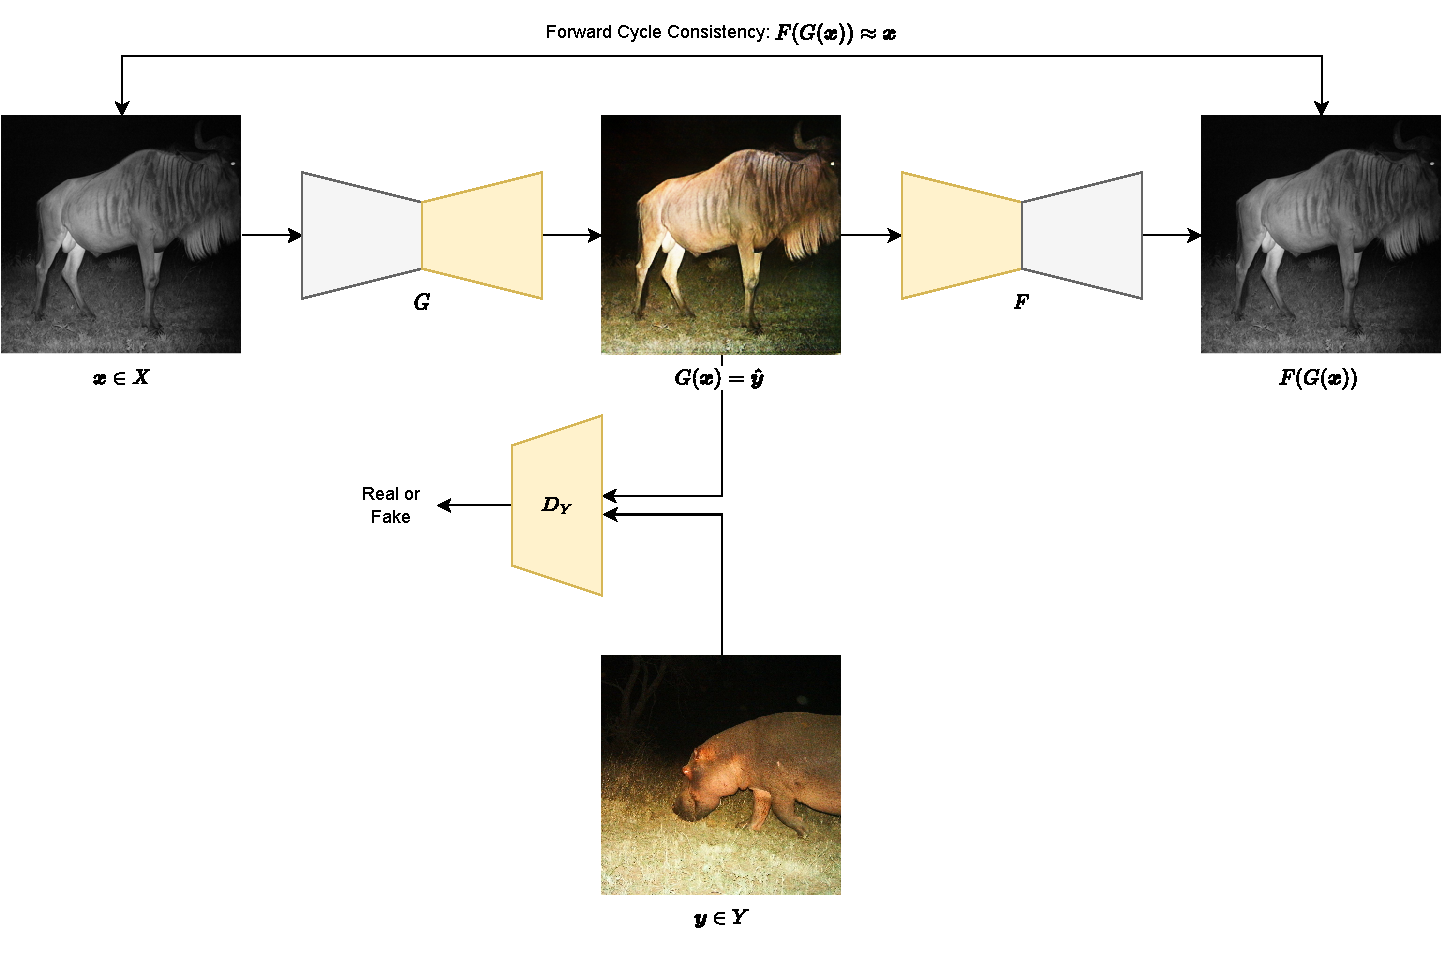
\includegraphics[width=\textwidth]{gfx/CycleGAN.pdf}
   \caption{
      \textbf{CycleGAN Schema.} Two generators $G$ and $F$ translate between both domains. Forward Cycle Consistency is ensured using the input and recovered NIR image.
      The discriminator $D_Y$ encourages the generator $G$ to learn the features of domain $\mathcal{Y}$ \parencite{cyclegan-original,mehri}.
   }
   \label{fig:cycle-gan}
\end{figure}

\subsubsection*{Cycle Consistency Loss}
This objective is written as a loss function $\mathcal{L}_{cyc}(G, F)$ which uses an L1 norm to encourage cycle consistency (\autoref{eqn:cyc}).
In addition to \textit{forward cycle consistency}, CycleGAN also utilizes \textit{backward cycle consistency} which means that for $\y \in \mathcal{Y}$, $G(F(\y)) \approx \y$ \parencite{cyclegan-original} applies, too (\autoref{fig:cycle-gan}).

\begin{equation}
   \label{eqn:cyc}
   \begin{aligned}
      \mathcal{L}_{cyc}(G, F) = \underbrace{\mathbb{E}_{\x \sim X}\left[||F(G(\x)) - \x||_1\right]}_{\text{forward cycle consistency}} +
      \underbrace{\mathbb{E}_{\y \sim Y}\left[||G(F(\y))) - \y||_1\right]}_{\textit{backward cycle consistency}}
   \end{aligned}
\end{equation}

In addition to the L1 cycle consistency loss, \citeauthor*{mehri} propose using \textit{structural similarity index measurement} (SSIM) as the second cycle consistency loss \parencite{mehri}.
Contrary to the L1 loss, SSIM measures the differences between the images not by the absolute image intensity values but by comparing two images based on luminance-, contrast- and structural similarity \parencite{ssim}.

Using measurements for luminance $l(\y_1, \y_2)$, contrast $c(\y_1,\y_2)$ and structure comparison $s(\y_1, \y_2)$, we can obtain the overall structural similarity
index $SSIM(\y_1, \y_2)$ as multiplication of each component (\autoref{eqn:ssim}) \parencite{ssim}.

\begin{equation}
   \label{eqn:ssim}
   \begin{aligned}
      SSIM(\y_1, \y_2) = l(\y_1, \y_2) \cdot c(\y_1,\y_2) \cdot s(\y_1, \y_2)
   \end{aligned}
\end{equation}

The SSIM is obtained using a moving Gaussian window on the image, and therefore the SSIM \textbf{difference} between two images $\overline{SSIM(\y_1,\y_2)}$ is calculated as follows (\autoref{eqn:ssim_difference}).
Let $\y_{1,j}$ and $\y_{2,j}$ be the image contents of the $j$-th local patch using the Gaussian window, where $M$ is the number of Gaussian windows.

\begin{equation}
   \label{eqn:ssim_difference}
   \begin{aligned}
      \overline{SSIM(\y_1,\y_2)} = \frac{1}{M}\sum_{j=1}^{M}1 - SSIM(\y_{1,j},\y_{2,j})
   \end{aligned}
\end{equation}

Finally, the loss of cycle consistency $\mathcal{L}_{SSIM}(G, F)$ can be constructed using the differences in the SSIMs between the images (\autoref{eqn:ssim_loss}).

\begin{equation}
   \label{eqn:ssim_loss}
   \begin{aligned}
      \mathcal{L}_{SSIM}(G,F) & = \mathbb{E}_{\x \sim X}\left[\overline{SSIM(F(G(\x)), \x)}\right] + \mathbb{E}_{\y \sim Y}\left[\overline{SSIM(G(F(\y)), \y)}\right]
   \end{aligned}
\end{equation}


\subsubsection*{Relativistic Adversarial Loss}
For both generators, adversarial discriminators $D_X$ and $D_Y$ are introduced where $D_X$ has the aim of distinguishing between real images
$X$ and generated images $\{F(\y)\}$ and $D_Y$ for $Y$ and $\{G(\x)\}$.
For both, we apply a relativistic GAN, in particular, \textit{RaLSGAN} \parencite{mehri,rel_gan}.
\autoref{eqn:ralsgan} demonstrates the RaLSGAN loss for the generator $G$ ($\mathcal{L}^G_{RaLSGAN}(G,D_Y,X,Y)$) and its discriminator
$D_Y$ ($\mathcal{L}^D_{RaLSGAN}(G,D_Y,X,Y)$) (\autoref{fig:cycle-gan}). The loss for $F$ and $D_X$ is defined in the same way as for $G$ and $D_Y$ \parencite{rel_gan}.

\begin{equation}
   \label{eqn:ralsgan}
   \begin{aligned}
      \mathcal{L}^{D_Y}_{RaLSGAN}(G,D_Y,X,Y) & = \mathbb{E}_{\y \sim Y}\left[(D_Y(\y) - \mathbb{E}_{\x \sim X} D_Y(G(\x)) - 1)^2 \right] \\
                                             & + \mathbb{E}_{\x \sim X}\left[(D_Y(G(\x)) - \mathbb{E}_{\y \sim Y} D_Y(\y) + 1)^2 \right] \\
      \mathcal{L}^G_{RaLSGAN}(G,D_Y,X,Y)     & = \mathbb{E}_{\x \sim X}\left[(D_Y(G(\x)) - \mathbb{E}_{\y \sim Y} D_Y(\y) - 1)^2 \right] \\
                                             & + \mathbb{E}_{\y \sim Y}\left[(D_Y(\y) - \mathbb{E}_{\x \sim X} D_Y(G(\x)) + 1)^2 \right]
   \end{aligned}
\end{equation}

\subsection*{Identity Loss}
Lastly, the identity loss has the aim of regulating the generator:
If an image already appears like a colored RGB image, it should not be modified.
This leads to the identity loss $\mathcal{L}_{identiy}$ (\autoref{eqn:identity_loss}) \parencite{mehri}.

\begin{equation}
   \label{eqn:identity_loss}
   \begin{aligned}
      \mathcal{L}_{identiy}(G, F) = \mathbb{E}_{\x \sim X} \left[||G(\x) - \x||_1\right] + \mathbb{E}_{\y \sim Y} \left[||G(\y) - \y||_1\right]
   \end{aligned}
\end{equation}

\subsection*{Full Objective}
All those four loss functions lead to an additive final loss function (\autoref{eqn:cycle_gan_total_loss}) \parencite{mehri}.
$\lambda$ and $\gamma$ are weights for the relative importance of the L1 cycle consistency loss and the identity loss.

\begin{equation}
   \label{eqn:cycle_gan_total_loss}
   \begin{aligned}
      \mathcal{L} = \lambda \mathcal{L}_{cyc} + \mathcal{L}_{SSIM} + \gamma \mathcal{L}_{identity}(G,F) + \mathcal{L}_{RaLSGAN}^G(G,D_Y,X,Y) + \mathcal{L}_{RaLSGAN}^F(F,D_X,Y,X)
   \end{aligned}
\end{equation}
% TIMM: sicherstellen dass die Gleichung umbricht

\subsubsection*{U-Net}
\label{sec:cycle-gan-u-net}
Typically, both functions $G$ and $F$ are generation networks. Contrary to the ResNet generators \parencite{resnet} \citeauthor{cyclegan-original} used in the original CycleGAN \parencite{cyclegan-original},
\citeauthor*{mehri} propose U-Net generators \parencite{unet}, because they perform better in learning the color \parencite{mehri}.
Additionally, U-Net generators also need less computational time for training compared to ResNet \parencite{mehri}.
We input all three (equal) channels of the NIR image into the generator and receive an RGB image as output.
All activations of the encode-blocks (except the last one) are inputs for two blocks:
The following encode- as well as the corresponding decode-block. This is called a skip connection \parencite{unet} (\autoref{fig:unet}). 
All decode-blocks (except the first one) receive input from the previous decode-block, as well as the corresponding encode-block.
Each encode-block consists of residual-blocks and downsample-blocks while all decode-blocks have upsample-blocks instead \parencite{unet}. 
Conceptually, the most abstract information can be found at the bottleneck (between encode and decode) and the most concrete information is located near the input and output of the model.
Through the skip connection the architecture that can learn to "choose" how deep the feature abstraction should be \parencite{unet}.

\begin{figure}[h]
   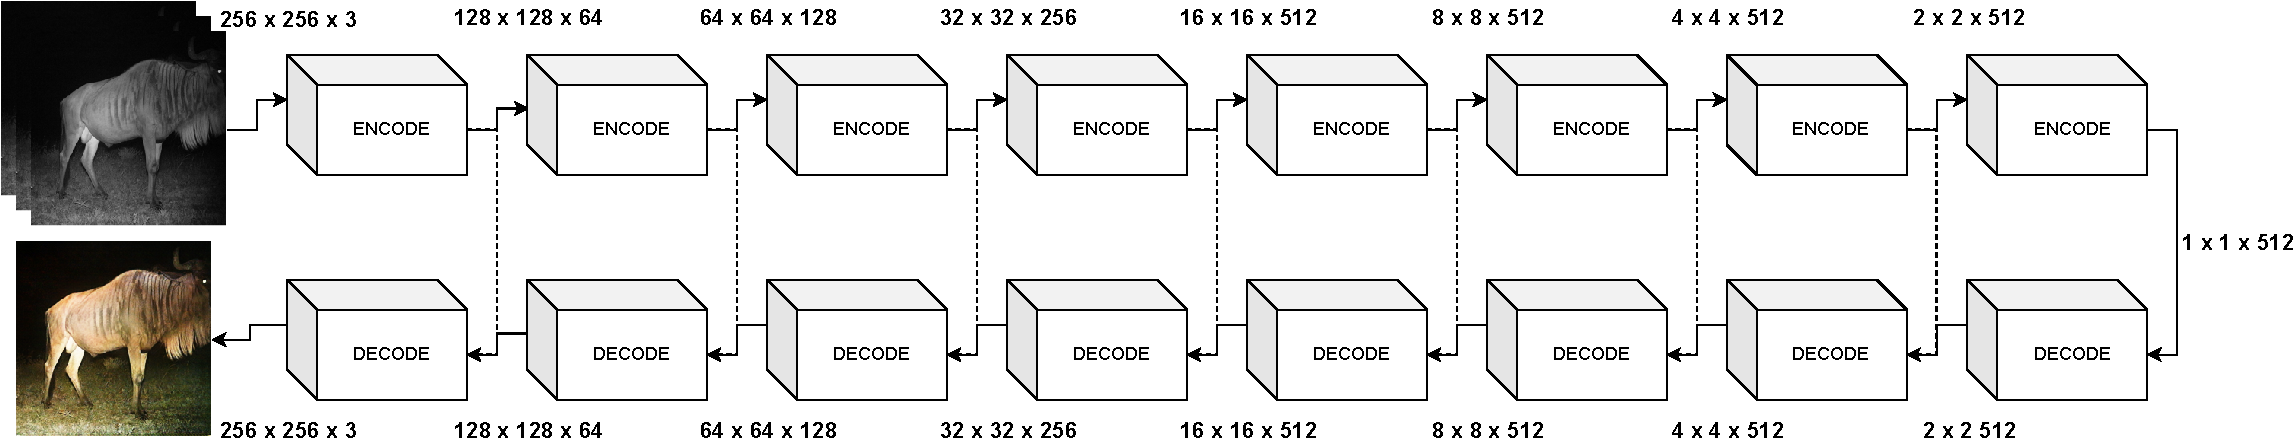
\includegraphics[width=\textwidth]{gfx/CycleGAN-Unet.pdf}
   \caption{
      \textbf{U-Net generator $G$ used in CycleGAN} \parencite{unet,mehri}.
   }
   \label{fig:unet}
\end{figure}

\subsubsection*{Optimizations}
\Citeauthor*{ttur} demonstrated that using the \textit{two timescale update rule} (TTUR) is beneficial, which states that when the generator and the discriminator have different learning rates,
mode collapse can be prevented in image translation tasks using GANs \parencite{ttur}. % TIMM: Satz bitte nochmal überprüfen
Inspired by this, \citeauthor*{mehri} propose utilizing two learning rates for the CycleGAN architecture \parencite{mehri}.

Additionally, \citeauthor*{mehri} propose the use of \textit{spectral normalization}, a technique introduced by \Citeauthor*{spectral-norm}, to stabilize the training of the discriminators $D_X$ and $D_Y$ \parencite{spectral-norm, mehri}.

Finally, \citeauthor*{mehri} observe that while the cycle consistency loss helps in the early training stages, it hinders the network in the later stages in generating realistic images \parencite{mehri}.
Therefore, \citeauthor*{mehri} propose to decrease the weight of the cycle consistency loss after half of the training process \parencite{mehri}.

\section{Diffusion Models}
Denoising Diffusion Probabilistic Models (DDPMs) as introduced by \cite{ddpm} are recent advances in the field of image generation.
We provide a detailed theoretical background for this architecture in \autoref{sec:diffusion-prerequisites}.
Further we answer theoretically how one can use unconditional diffusion to sample given a condition in \autoref{sec:conditional-sampling}.
Our approach for grayscale-colorization and near-infrared colorization is presented in \autoref{sec:correction-guided-sampling} while
we introduce at first sight simpler formulation using what we call \textit{energy-guided conditional sampling} in \autoref{sec:energy-guided-sampling}.

\subsection{Prerequisites}
\label{sec:diffusion-prerequisites}
Our diffusion process consists of $T$ timesteps.
$\x_0$ is the original image and $\x_T$ is the final noised image following an isotropic Gaussian distribution.

With $q(\x_t | \x_{t-1})$ we denote the \textit{forward process}, which describes the distribution of $\x_t$ given a less noised $\x_{t-1}$:
The forward process gradually adds Gaussian noise to the image determined by the \textit{variance schedule} $\beta_1, \dots, \beta_T$ \parencite[\autoref{eqn:forward-process-definition}]{ddpm}.

\begin{equation}
   \label{eqn:forward-process-definition}
   \begin{aligned}
      q(\mathbf{x}_t | \x_{t-1}) := & \mathcal{N}(\x_t; \sqrt{1 - \beta_t}\x_{t-1}, \beta_t \mathbf{I})                                            \\
      \Rightarrow \x_t =            & \sqrt{1 - \beta_t}\x_{t-1} + \sqrt{\beta_t} \epsilon              & \epsilon \sim \mathcal{N}(0, \mathbb{I})
   \end{aligned}
\end{equation}

To sample $\x_t \sim q(\x_t | \x_0)$, repeatedly sampling is not necessary, a closed form can be derived (\autoref{eqn:forward-process-closed-form}),
while defining $\alpha_t := 1 - \beta_t$ and $\bar\alpha_t := \prod_{s=1}^t \alpha_s$ \parencite{ddpm}.

\begin{equation}
   \label{eqn:forward-process-closed-form}
   \begin{aligned}
      q(\x_t|\x_0)     & = \mathcal{N}(\x_t; \sqrt{\bar{\alpha}_t}\x_{0}, (1 - \bar{\alpha}_t) \mathbf{I})                                            \\
      \Rightarrow \x_t & = \sqrt{\bar{\alpha}_t}\x_{0} + \sqrt{1 - \bar{\alpha}_t} \epsilon                & \epsilon \sim \mathcal{N}(0, \mathbb{I})
   \end{aligned}
\end{equation}

The posterior $q(\x_{t-1}|\x_t, \x_0)$ can also be expressed as Gaussian $\mathcal{N}(\x_{t-1}; \tilde{\mu}(\x_t, \x_0), \tilde{\beta}_t\mathbf{I})$ where mean $\tilde{\mu}(\x_t, \x_0)$ and variance $\tilde{\beta}_t$
are derivable using the Bayes theorem resulting in \autoref{eqn:mu-and-beta} \parencite{ddpm}.

\begin{equation}
   \label{eqn:mu-and-beta}
   \begin{aligned}
      \tilde{\mu}(\x_t, \x_0) & := \frac{\sqrt{\bar{\alpha}_{t-1}}\beta_t}{1 - \bar{\alpha}_{t}}\x_0 + \frac{\sqrt{\alpha_t}(1 - \bar{\alpha}_{t-1})}{1 - \bar{\alpha}_{t}}\x_t                                                            \\
                              & = \frac{1}{\sqrt{\alpha_t}} \left(\x_t - \frac{\beta_t}{\sqrt{1 - \bar{\alpha}_t}} \epsilon_t \right)                                           & \text{where } \epsilon_t \sim \mathcal{N}(0, \mathbf{I}) \\
      \tilde{\beta}_t         & := \frac{1 - \bar{\alpha}_{t-1}}{1 - \bar{\alpha}_t} \beta_t
   \end{aligned}
\end{equation}

Sampling using a DDPM is then reversing this process.
First a sample is obtained from the prior distribution $q(\x_T)$ which
is nearly an isotropic Gaussian, therefore $\x_T \sim \mathcal{N}(0, \mathbf{I})$.
Then we gradually \textit{denoise} our sample using $q(\x_{t-1}|\x_t)$ until $t = 0$.
Because $q(\x_{t-1}|\x_t)$ is not trivial obtainable without knowing the data distribution,
we leverage a neural network $p_\theta$ to approximate it.
$\theta$ denote the parameters of the network.
If $\beta_t$ is small enough it will also be Gaussian (\autoref{eqn:reverse-process}) \parencite{ddpm}.

\begin{equation}
   \label{eqn:reverse-process}
   \begin{aligned}
      p_\theta(\x_{t-1}|\x_t) & := \mathcal{N}(\x_{t-1};\mu_\theta(\x_t,t), \Sigma_\theta(\x_t,t))                                            \\
      \Rightarrow \x_{t-1}    & = \mu_\theta(\x_t,t) + \sqrt{||\Sigma_\theta(\x_t,t)||} \epsilon   & \epsilon \sim \mathcal{N}(0, \mathbf{I})
   \end{aligned}
\end{equation}

To train the neural network, one wants to minimize the log-likelihood $-\log p_\theta(\x_0)$.
As this is difficult to train, a variational lower bound using the Kullback-Leibler divergence can be leveraged (\autoref{eqn:loss-vlb}) \parencite{ddpm}.

\begin{equation}
   \label{eqn:loss-vlb}
   \begin{aligned}
             & -\log p_\theta(\x_0)                                                                                                                                                                                                           \\
      \leq   & -\log p_\theta(\x_0) + D_{KL}(q(\x_{1:T}|\x_0) || p_\theta(\x_{1:T}|\x_0))                                                                                                                                                     \\
      =      & \mathbb{E}_q\left[\log\left(\frac{q(\x_{1:T}|\x_0)}{p_\theta(\x_{0:T})}\right)\right]                                                                                                                                          \\
      =      & \mathbb{E}_q\left[\log\left(\frac{\prod_{t=1}^Tq(\x_t|\x_{t-1})}{p_\theta(\x_T)\prod_{t=1}^Tp_\theta(\x_{t-1}|\x_t)}\right)\right]                                                                                             \\
      =      & \mathbb{E}_q\left[\log\left(\frac{\prod_{t=1}^Tq(\x_t|\x_{t-1})}{p_\theta(\x_T)\prod_{t=1}^Tp_\theta(\x_{t-1}|\x_t)}\right)\right]                                                                                             \\
      \vdots &                                                                                                                                                                                                                                \\
      =      & \mathbb{E}_q\left[ \underbrace{D_{KL}(q(\x_T|\x_0)||p_\theta(\x_T))}_{L_T} + \sum_{t=2}^T \underbrace{D_{KL}(q(\x_{t-1}|\x_t,\x_0)||p_\theta(\x_{t-1}|\x_t))}_{L_{t-1}} \underbrace{ - \log p_\theta(\x_0|\x_1)}_{L_0} \right] \\
   \end{aligned}
\end{equation}

We minimize our objective by minimizing the additive terms $L_T$, $L_{t-1}$ for all $t \in [2:T]$ and $L_0$.
As $L_T$ is constant this can be ignored during training.
Because every $D_{KL}$ term compares two Gaussian distributions, they can be computed in closed form.
We can rewritte the term $L_{t-1}$ as \autoref{eqn:loss-t-1} where $C$ is a constant independent of $\theta$ and can therefore be ignored while minimizing.

\begin{equation}
   \label{eqn:loss-t-1}
   L_{t-1}=\mathbb{E}_q\left[\frac{1}{2||\Sigma_\theta(\x_t,t)||_2^2}||\tilde{\mu}_t(\x_t,\x_0) - \mu_\theta(\x_t,t)||^2\right] + C
\end{equation}

This equation can be further expanded by utilizing \autoref{eqn:forward-process-closed-form} and \autoref{eqn:mu-and-beta}:

\begin{equation}
   L_{t-1} - C =\mathbb{E}_q\left[\frac{1}{2||\Sigma_\theta(\x_t,t)||_2^2}|| \frac{1}{\sqrt{\alpha_t}} \left(\x_t - \frac{\beta_t}{\sqrt{1 - \bar{\alpha}_t}} \epsilon_t \right) - \mu_\theta(\x_t,t)||^2\right]
\end{equation}

Because this reveals that $\mu_\theta$ must predict $\frac{1}{\sqrt{\alpha_t}} \left(\x_t - \frac{\beta_t}{\sqrt{1 - \bar{\alpha}_t}} \epsilon_t \right)$ given $\x_t$ to minimize the loss,
\textcite{ddpm} choose to parameterize $\mu_\theta(\x_t, t)$ as follows, where $\epsilon_\theta$ is a function to predict $\epsilon$ given $\x_t$ (\autoref{eqn:mu-theta-parameterization}).

\begin{equation}
   \label{eqn:mu-theta-parameterization}
   \mu_\theta(\x_t, t) = \frac{1}{\sqrt{\alpha_t}} \left(\x_t - \frac{\beta_t}{\sqrt{1 - \bar{\alpha}_t}} \epsilon_t \right)
\end{equation}

With parameterization \autoref{eqn:mu-and-beta}, the loss can be simplified as \autoref{eqn:epsilon-parameterized-loss}, as proposed by \textcite{ddpm}.

\begin{equation}
   \label{eqn:epsilon-parameterized-loss}
   \mathbb{E}_{\x_0, \epsilon}\left[ \frac{\beta_t^2}{2 ||\Sigma_\theta(\x_t,t)||_2^2 \alpha_t(1-\bar{\alpha}_t)} || \epsilon - \epsilon_\theta(\sqrt{\bar{\alpha}_t}\x_0 + \sqrt{1 - \bar{\alpha}_t} \epsilon,t) ||^2 \right]
\end{equation}

Furthermore, \textcite{ddpm} found, that when not learning $\Sigma_\theta$, and fixing it by the beta-schedule, the loss \autoref{eqn:simple-loss} is even better for sample quality and is easier to implement.
To be precise \textcite{ddpm} fix $\Sigma_\theta(\x_t, t) = \sigma_t^2\mathbf{I}$ with either $\sigma_t^2 = \beta_t$ or $\sigma_t^2 = \tilde{\beta}_t$.

\begin{equation}
   \label{eqn:simple-loss}
   L_{simple}(\theta) := \mathbb{E}_{t \sim [1,T], \x_0, \epsilon_t}\left[ || \epsilon_t - \epsilon_\theta(\sqrt{\bar{\alpha}_t}\x_0 + \sqrt{1 - \bar{\alpha}_t} \epsilon,t)  ||^2 \right]
\end{equation}

By this the training algorithm for this \textit{unconditional} can be derived as \autoref{alg:training} \parencite{ddpm}.

\begin{algorithm}[htp!]
   \caption{Training \parencite{ddpm}}
   \label{alg:training}
   \begin{algorithmic}
      \Repeat
      \State $\x_0 \sim q(\x_0)$
      \State $t \sim \mathrm{Uniform}(\{1, \dots, T\})$
      \State $\epsilon \sim \mathcal{N}(0, \mathbf{I})$
      \State Take gradient step on $\nabla_\theta || \epsilon_t - \epsilon_\theta(\sqrt{\bar{\alpha}_t}\x_0 + \sqrt{1 - \bar{\alpha}_t} \epsilon,t) ||^2$
      \Until{converged}
   \end{algorithmic}
\end{algorithm}



Sampling with this unconditional model (\autoref{alg:sampling-unconditional}) then uses the reparameterization of the Gaussian distribution (\autoref{eqn:reverse-process})
and the parameterization of the mean given an $\epsilon$ predicted by the model (\autoref{eqn:mu-theta-parameterization}) \parencite{ddpm}.
This process is also visualized in \autoref{fig:reverse-diffusion-process}.


\begin{algorithm}[htp!]
   \caption{Unconditional Sampling \parencite{ddpm}}
   \label{alg:sampling-unconditional}
   \begin{algorithmic}
      \State $\x_T \sim \mathcal{N}(0, \mathbf{I})$
      \For{$t = T, \dots, 1$}
      \State $\mathbf{z} \sim \mathcal{N}(0, \mathbf{I})$ \algorithmicif\ $t > 0$, \algorithmicelse\ $\mathbf{z} = 0$
      \State $\x_{t-1} = \frac{1}{\sqrt{\alpha_t}} \left(\x_t - \frac{\beta_t}{\sqrt{1 - \bar{\alpha}_t}} \epsilon_\theta(\x_t, t) \right) + \sigma_t \mathbf{z}$
      \EndFor
      \Return $\x_0$
   \end{algorithmic}
\end{algorithm}

\begin{figure}[htp!]
   \centering
   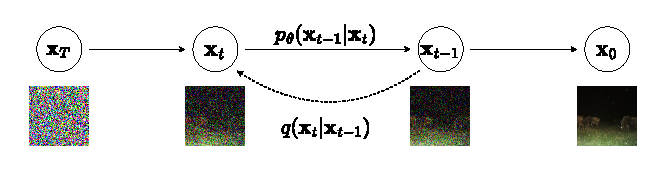
\includegraphics[width=.8\textwidth]{gfx/Unconditional-Sampling.pdf}
   \caption{
      \textbf{Reverse Diffusion Process.}
      Starting from $\x_T$ sampled from a prior distribution, we gradually remove noise from the image using $p_\theta(\x_{t-1}|\x_t)$ until $\x_0$ is reached.
      $q(\x_t | \x_{t-1})$ denotes the forward diffusion process and is the counterpart to $p_\theta(\x_{t-1}|\x_t)$, used for training and theoretical derivation \parencite{ddpm}.
   }
   \label{fig:reverse-diffusion-process}
\end{figure}


\todo{Structural comparison with CycleGAN}

Similar to CycleGAN, diffusion models utilize the U-Net architecture for learning the noise $\epsilon_\theta(\x_t,t)$ \parencite{unet,mehri,ddpm,diffusion-beats-gans} (see \autoref{sec:cycle-gan-u-net}).
Additionally, \cite{diffusion-beats-gans} use global attention blocks.  
Unlike CycleGAN, the model needs information about the timestep $t$. This is provided using sinusoidal position embedding into the residual blocks \parencite{ddpm}.

\subsection{Conditional Sampling}
\label{sec:conditional-sampling}
Our application context of NIR colorization is not able to benefit from the unconditional sampling as derived up until now.
A method is needed to \textit{condition} our diffusion model on the given NIR image.
We now derive a general purpose conditioning method as \textcite{sbgm,diffusion-beats-gans} introduced them and show in \autoref{sec:correction-guided-sampling} and \autoref{sec:energy-guided-sampling}
two different way of leveraging to achieve our goal.

Given a Gaussian distribution $p(\x) = \mathcal{N}(\x, \mu, \sigma^2 \mathbf{I})$ the derivative of the density function $\nabla_\x \log p(\x)$, called \textit{score-function} can be rewritten as in \autoref{eqn:score-function} for an $\epsilon \sim \mathcal{N}(0, \mathbf{I})$ \parencite{sbgm}.

\begin{equation}
   \label{eqn:score-function}
   \nabla_\x \log p(\x) = \nabla_\x \left( - \frac{1}{2\cdot\sigma^2}(\x-\mu)^2\right) = - \frac{\x - \mu}{\sigma^2} = - \frac{\epsilon}{\sigma^2}
\end{equation}

If we would now calculate the score-function of our reverse process $p_\theta(\x_t)$ (\autoref{eqn:reverse-process})
we find a connection between score-functions and our noise estimator network \parencite{sbgm}, see \autoref{eqn:score-function-p}.

\begin{equation}
   \label{eqn:score-function-p}
   \nabla_{\x_t} \log p_\theta(\x_t) = - \frac{\epsilon_\theta(\x_t, t)}{\sqrt{1 - \bar{\alpha}_t}}
\end{equation}

If we want now to sample using a condition $\ce$, then we would need to sample from the distribution $p_\theta(\x_t | \ce)$ each iteration.
To be able to sample from this distribution we can derive an new noise estimator $\bar{\epsilon}_\theta(\x_t, \ce, t)$ which
separates the conditioning $p_\theta(\ce|\x_t)$ and the unconditional noise estimator $\epsilon_\theta(\x_t, t)$ (\autoref{eqn:derive-new-noise-estimator}) \parencite{sbgm,diffusion-beats-gans}.

\begin{equation}
   \label{eqn:derive-new-noise-estimator}
   \begin{aligned}
      \nabla_{\x_t} \log p_\theta(\x_t|\ce)           & = \nabla_{\x_t} \log p_\theta(\x_t|\ce)                                                                                                                                                           \\
                                                      & = \nabla_{\x_t} \log \left( \frac{p_\theta(\x_t) \cdot p_\theta(\ce|\x_t)}{p_\theta(\ce)} \right)                                                                                                 \\
                                                      & = \nabla_{\x_t} \left( \log p_\theta(\x_t) + \log p_\theta(\ce|\x_t) - p_\theta(\ce) \right)                                                                                                      \\
                                                      & = \nabla_{\x_t} \log p_\theta(\x_t) + \nabla_{\x_t} \log p_\theta(\ce|\x_t)                                                                                                                       \\
                                                      & =  - \frac{\epsilon_\theta(\x_t, t)}{\sqrt{1 - \bar{\alpha}_t}} + \nabla_{\x_t} \log p_\theta(\ce|\x_t)                                                                                           \\
                                                      & = -\frac{1}{\sqrt{1 - \bar{\alpha}_t}} \underbrace{\left(\epsilon_\theta(\x_t, t) - \sqrt{1 - \bar{\alpha}_t} \nabla_{\x_t} \log p_\theta(\ce|\x_t)\right)}_{\bar{\epsilon}_\theta(\x_t, \ce, t)} \\
                                                      & = -\frac{\bar{\epsilon}_\theta(\x_t, \ce, t)}{\sqrt{1 - \bar{\alpha}_t}}                                                                                                                          \\
      \\
      \Rightarrow \bar{\epsilon}_\theta(\x_t, \ce, t) & = \epsilon_\theta(\x_t, t) - \sqrt{1 - \bar{\alpha}_t} \nabla_{\x_t} \log p_\theta(\ce|\x_t)
   \end{aligned}
\end{equation}

By using this new noise estimator $\bar{\epsilon}_\theta(\x_t, \ce, t)$, we can sample new images with the condition using \autoref{alg:sampling-unconditional}: 

\begin{equation}
   \begin{aligned}
      \x_{t-1} &= \frac{1}{\sqrt{\alpha_t}} \left(\x_t - \frac{\beta_t}{\sqrt{1 - \bar{\alpha}_t}} \bar{\epsilon}_\theta(\x_t, \ce, t) \right) + \sigma_t \mathbf{z} \\
      &= \frac{1}{\sqrt{\alpha_t}} \left(\x_t - \frac{\beta_t}{\sqrt{1 - \bar{\alpha}_t}} (\epsilon_\theta(\x_t, t) - \sqrt{1 - \bar{\alpha}_t} \nabla_{\x_t} \log p_\theta(\ce|\x_t)) \right) + \sigma_t \mathbf{z} \\
      &= \underbrace{\frac{1}{\sqrt{\alpha_t}} \left(\x_t - \frac{\beta_t}{\sqrt{1 - \bar{\alpha}_t}} \epsilon_\theta(\x_t, t) \right) + \sigma_t \mathbf{z}}_{\tilde{\x}_{t-1}} + \frac{\beta_t}{\sqrt{\alpha_t}} \nabla_{\x_t} \log p_\theta(\ce|\x_t) \\
      &= \tilde{\x}_{t-1} + \frac{\beta_t}{\sqrt{\alpha_t}} \nabla_{\x_t} \log p_\theta(\ce|\x_t) \\
   \end{aligned}
\end{equation}

Therefore, it is possible to use a general purpose unconditional diffusion model and conditional sample with it.
It is only needed to calculate or approximate the score-function $\nabla_{\x_t} \log p_\theta(\ce|\x_t)$ \parencite{diffusion-beats-gans}.
\autoref{alg:sampling-conditional} shows how conditional sampling can be implemented.

\begin{algorithm}[htp!]
   \caption{Conditional Sampling}
   \label{alg:sampling-conditional}
   \begin{algorithmic}
      \Require A score-function $\nabla_{\x_t} \log p_\theta(\ce|\x_t)$ modeling the derivative of the log of the density function to the condition $\ce$ given a noised image $\x_t$.
      \State $\x_T \sim \mathcal{N}(0, \mathbf{I})$
      \For{$t = T, \dots, 1$}
      \State $\mathbf{z} \sim \mathcal{N}(0, \mathbf{I})$ \algorithmicif\ $t > 0$, \algorithmicelse\ $\mathbf{z} = 0$
      \State $\tilde{\x}_{t-1} = \frac{1}{\sqrt{\alpha_t}} \left(\x_t - \frac{\beta_t}{\sqrt{1 - \bar{\alpha}_t}} \epsilon_\theta(\x_t, t) \right) + \sigma_t \mathbf{z}$
      \State $\x_{t-1} = \tilde{\x}_{t-1} + \frac{\beta_t}{\sqrt{\alpha_t}} \nabla_{\x_t} \log p_\theta(\ce|\x_t)$
      \EndFor
      \Return $\x_0$
   \end{algorithmic}
\end{algorithm}

\subsection{Correction-Guided Conditional Sampling}
\label{sec:correction-guided-sampling}

We consider \textit{correction-guided sampling} a specialized form of the conditional sampling as derived in \autoref{sec:conditional-sampling}.
Conceptually each iteration we \textit{correct} the image after the sampling to be consistent with the condition property -- in our case the near-infrared image.
Therefore, we now sample in each iteration a $\tilde{\x}_{t-1} \sim p_\theta(\tilde{\x}_{t-1}| \x_{t})$ as before, but use a correction function $f(\tilde{\x}_{t-1}, \ce)$ which ensures the condition property $\ce$.
Leveraging this function, we obtain the corrected image $\x_{t-1} = f(\tilde{\x}_{t-1}, \ce)$, which is input for the next iteration. 

This procedure is equivalent to using a conditional score function $\nabla_{\x_t}\log p_\theta(\ce | \x_{t})$ as in \autoref{eqn:correction-guided-sampling-score-function}.
Note that we use different indices on the score function and the correction term. 
Even though originally this is derived using $\x_{t}$, we correct using the newest generated image $\tilde{\x}_{t-1}$.  

\begin{equation}
   \label{eqn:correction-guided-sampling-score-function}
   \nabla_{\x_t}\log p_\theta(\ce | \x_{t}) = \frac{\sqrt{\alpha_t}}{\beta_t}(f(\tilde{\x}_{t-1}, \ce) - \tilde{\x}_{t-1}) 
\end{equation}

We note that \textcite{ilvr} use a similar technique which they call iterative latent variable refinement, but they do not present this mathematical connection. 

In \autoref{alg:sampling-conditional-correction-guided} we present our algorithm for correction-guided sampling.

\begin{algorithm}[htp!]
   \caption{Correction-Guided Conditional Sampling}
   \label{alg:sampling-conditional-correction-guided}
   \begin{algorithmic}
      \Require A correction function $f$ ensuring the condition $\ce$ given a noised image $\x_t$.
      \State $\x_T \sim \mathcal{N}(0, \mathbf{I})$
      \For{$t = T, \dots, 1$}
      \State $\mathbf{z} \sim \mathcal{N}(0, \mathbf{I})$ \algorithmicif\ $t > 0$, \algorithmicelse\ $\mathbf{z} = 0$
      \State $\tilde{\x}_{t-1} = \frac{1}{\sqrt{\alpha_t}} \left(\x_t - \frac{\beta_t}{\sqrt{1 - \bar{\alpha}_t}} \epsilon_\theta(\x_t, t) \right) + \sigma_t \mathbf{z}$
      \State $\x_{t-1} = f(\tilde{\x}_{t-1}, \ce)$
      \EndFor
      \Return $\x_0$
   \end{algorithmic}
\end{algorithm}

For our concrete application context we derive two different formulations of the correction function $f(\tilde{\x}_t, \ce)$ and of the condition $\ce$ 
for colorizing gray-scale (\autoref{sec:correction-guided-sampling-gray-scale-colorization}) and near-infrared (\autoref{sec:correction-guided-sampling-nir-colorization}) images. 

\subsubsection{Gray-Scale Colorization}
\label{sec:correction-guided-sampling-gray-scale-colorization}

Colorization can also be considered as specialized form of \textit{image imputation} as \textcite{sbgm} showed.
Image imputation is the task of restoring lost parts of an image congruent with the known areas of the image.
In the case of grayscale-colorization the known part is the \textit{intensity} while unknown are the remaining dimensions for a colored image, e.g. \textit{hue} and \textit{saturation}.
Therefore, we first sample in each iteration $t-1$ a $\tilde{\x}_{t-1}$ from the diffusion model given $\x_t$ using $p_\theta(\tilde{\x}_{t-1}|\x_t)$.
Simultaneously, we diffuse our input image $\y_0$ to the timestep $t-1$ using $q(\y_{t-1}, \y_0)$.
We then decompose both images into their intensity parts $\tilde{\x}_{t-1}^I$, $\y_{t-1}^I$ and the remaining parts $\tilde{\x}_{t-1}^R$, $\y_{t-1}^R$ using \textproc{DecoupleIntensity}, so that no information is lost.
The noised input image's intensity $\y_{t-1}^I$ is then combined with the color information of the sample $\tilde{\x}_{t-1}^I$ and transformed back into the RGB domain using \textproc{CoupleIntensity} to obtain $\x_{t-1}$.
We implement this colorization approach according to \autoref{alg:sampling-gray-scale-colorization} and evaluate it for NIR colorization in \autoref{sec:nir-as-intensity-approximation-evaluation}.

\begin{algorithm}[htp!]
   \caption{Gray-Scale Colorization Sampling}
   \label{alg:sampling-gray-scale-colorization}
   \begin{algorithmic}
      \Require Reference gray-scale image $\y_0$
      \State $\x_T \sim \mathcal{N}(0, \mathbf{I})$
      \For{$t = T, \dots, 1$}
      \State $\y_{t-1} \sim q(\y_{t-1}| \y_0)$
      \State $\tilde{\x}_{t-1} \sim p_\theta(\x_{t-1}|\x_t)$
      \State $\y_{t-1}^I, \y_{t-1}^R = $\ \Call{DecoupleIntensity}{$\y_{t-1}$}
      \State $\tilde{\x}_{t-1}^I, \tilde{\x}_{t-1}^R=$\ \Call{DecoupleIntensity}{$\tilde{\x}_{t-1}$}
      \State $\x_{t-1}=$ \ \Call{CoupleIntensity}{$\y_{t-1}^I$,$\tilde{\x}_{t-1}^R$}
      \EndFor
      \Return $\x_0$
   \end{algorithmic}
\end{algorithm}

\begin{figure}
   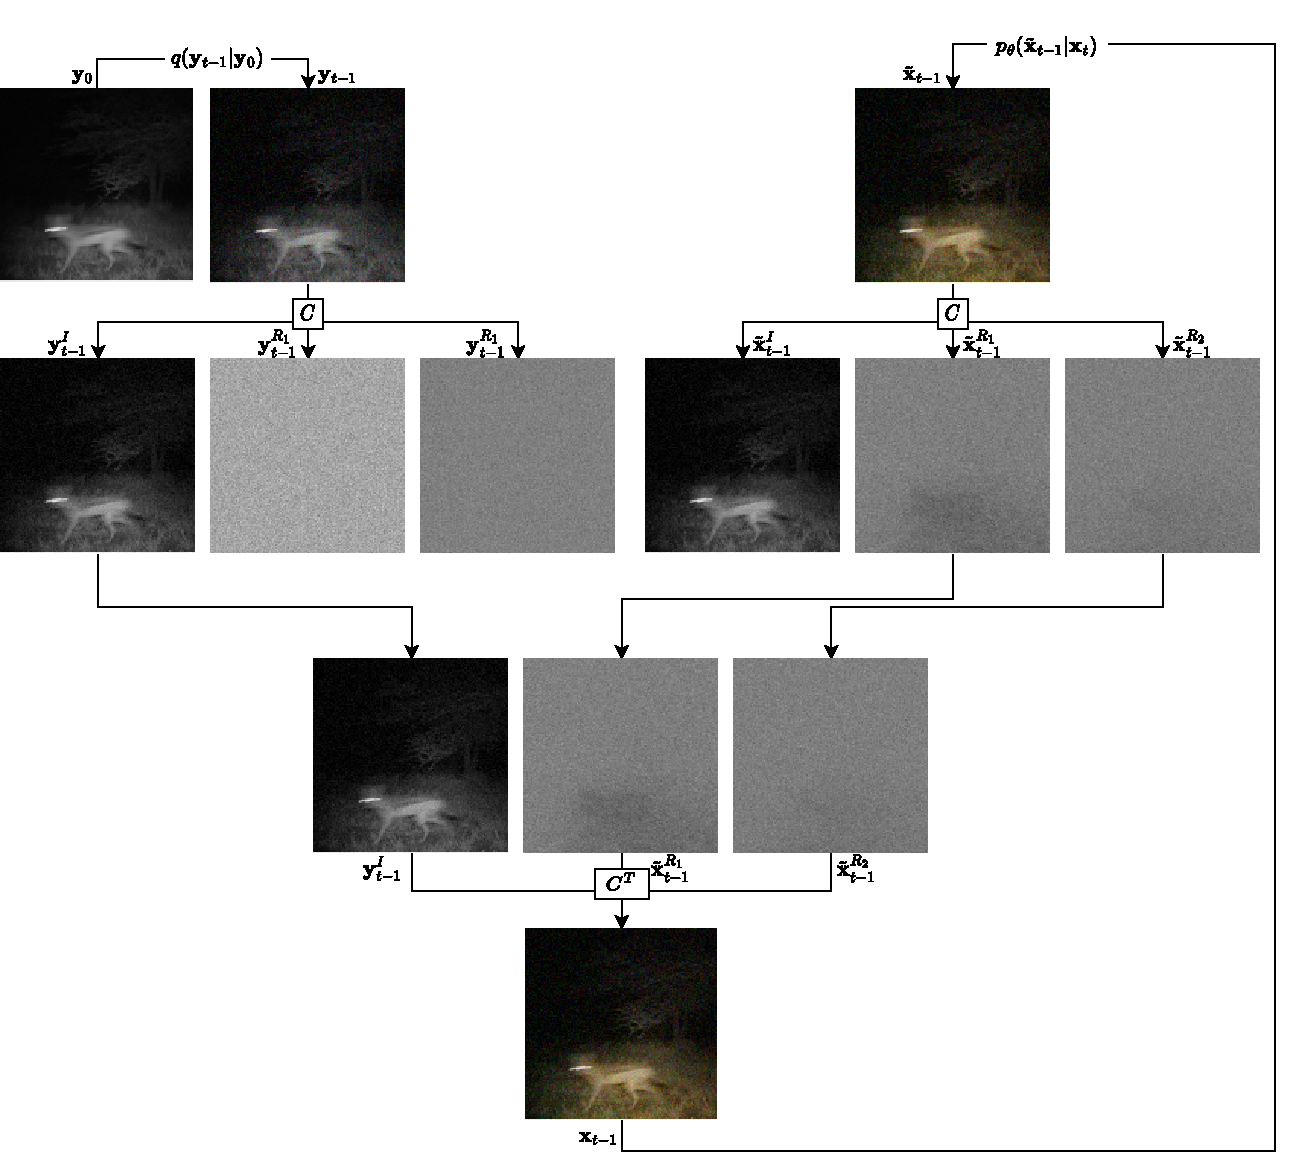
\includegraphics[width=\textwidth]{gfx/Gray-Scale-Colorization-Sampling.pdf}
   \caption{
      \textbf{Iteration Schema for Colorization using Intensity Replacement}.
      First approximate $\tilde{\x}_{t-1}$ and noised input image are $\y_{t-1}$ sampled with $p_\theta(\x_{t-1}|\x_t)$ and $q(\y_{t-1}|\y_0)$ respectively.
      Both are then decomposed into intensity and remaining dimensions. 
      Intensity of the noised input image $\y_{t-1}^I$ is combined with color of the approximate sample $\tilde{\x}_{t-1}^R$ and transformed back into regular RGB domain, obtaining $\x_{t-1}$ (\autoref{alg:sampling-gray-scale-colorization})
      $C$ denotes decomposition function into intensity and remaining dimensions.
   }
   \label{fig:sampling-gray-scale-colorization}
\end{figure}

We call this method \textit{correction-guided} sampling since we guide the sampling process by \textit{correcting} the sample in each iteration.

\textproc{DecoupleIntensity} and \textproc{CoupleIntensity} can theoretically be any invertible transformation where the intensity is decoupled from the color information.
Intuitive options would be color spaces such as HSI, HSV, LAB, YCbCr, \dots,
but we found empirically that transforming the RGB image using an orthogonal matrix where the resulting space's first dimension is the intensity to give best results:

Therefore, we search for a matrix $C \in \mathbb{R}^{3\times3}$ such that for any RGB pixel $p = \begin{pmatrix}r & g &b\end{pmatrix} \in \mathbb{R}^3$ and a fixed scalar $a \in \mathbb{R}$ the requirements of \autoref{eqn:requirements-c} are fulfilled.
\begin{equation}
   \label{eqn:requirements-c}
   \begin{aligned}
      p' & = p \cdot C \Rightarrow p'_1 = a \cdot (r + g + b) \\
      p  & = (p \cdot C) \cdot C^T
   \end{aligned}
\end{equation}

This can be obtained by a system of equations or QR decomposition. \todo{Check QR-decomposition statement.}
We derive the matrix $C$ as \autoref{eqn:matrix-c-used}, while \autoref{eqn:matrix-c-ref} is a different solution to the requirements as \textcite{sbgm} obtained it.

\begin{align}
   C_1 & =
   \begin{pmatrix}
      \frac{1}{\sqrt{3}} & - \sqrt{\frac{2}{3}} & 0                   \\
      \frac{1}{\sqrt{3}} & \frac{1}{\sqrt{6}}   & \frac{1}{\sqrt{2}}  \\
      \frac{1}{\sqrt{3}} & \frac{1}{\sqrt{6}}   & -\frac{1}{\sqrt{2}}
   \end{pmatrix}
   \approx
   \begin{pmatrix}
      0.577 & -0.816 & 0      \\
      0.577 & 0.408  & 0.707  \\
      0.577 & 0.408  & -0.707
   \end{pmatrix}
   \label{eqn:matrix-c-ref} \\
   C_2 & =
   \begin{pmatrix}
      \frac{1}{\sqrt{3}} & -\frac{1}{2} - \frac{1}{2\sqrt{3}} & \frac{1}{2} - \frac{1}{2\sqrt{3}}  \\
      \frac{1}{\sqrt{3}} & \frac{1}{2} - \frac{1}{2\sqrt{3}}  & -\frac{1}{2} - \frac{1}{2\sqrt{3}} \\
      \frac{1}{\sqrt{3}} & \frac{1}{\sqrt{3}}                 & \frac{1}{\sqrt{3}}
   \end{pmatrix}
   \approx
   \begin{pmatrix}
      0.577 & -0.789 & 0.211  \\
      0.577 & 0.211  & -0.789 \\
      0.577 & 0.577  & 0.577
   \end{pmatrix}
   \label{eqn:matrix-c-used}
\end{align}

\subsubsection{NIR Colorization}
\label{sec:correction-guided-sampling-nir-colorization}

We discover that this method of colorization near-infrared images does generate good results, but is too limited in the intensity:
By fixing the intensity to the near-infrared image's one, we ignore the different wave lengths and reflectance properties of the near-infrared light and visible light.
We observe intensities differences lie in the large areas rather than in the details \autoref{sec:nir-as-intensity-approximation-evaluation}.
This corresponds to difference in low-frequencies of the intensity while high-frequencies of the intensity are quite similar.
This property was also already used in the related research field of NIR-RGB image fusion \parencite{study-vis-nir-fusion},
and we use this as an inspiration for generating color.

To leverage this observation, we base our approach on \autoref{alg:sampling-gray-scale-colorization}.
However instead of simply using the intensity of the NIR image $\y_{t-1}^I$, we only use the high frequencies of the NIR's intensity $\y_{t-1}^{I_H}$
and combine them with the low-frequencies of the sample's intensity $\tilde{\x}_{t-1}^{I_L}$.
In \autoref{alg:sampling-nir-colorization} we demonstrate our general algorithm.

\begin{algorithm}[htp!]
   \caption{General NIR-Colorization Sampling}
   \label{alg:sampling-nir-colorization}
   \begin{algorithmic}
      \Require Reference NIR image $\y_0$
      \State $\x_T \sim \mathcal{N}(0, \mathbf{I})$
      \For{$t = T, \dots, 1$}
      \State $\y_{t-1} \sim q(\y_{t-1}| \y_0)$
      \State $\tilde{\x}_{t-1} \sim p_\theta(\x_{t-1}|\x_t)$
      \State $\y_{t-1}^I, \y_{t-1}^R = $\ \Call{DecoupleIntensity}{$\y_{t-1}$}
      \State $\tilde{\x}_{t-1}^I, \tilde{\x}_{t-1}^R=$\ \Call{DecoupleIntensity}{$\tilde{\x}_{t-1}$}
      \State $\tilde{\x}_{t-1}^{I_L}, \tilde{\x}_{t-1}^{I_H} =$\ \Call{DecomposeFrequencies}{$\tilde{\x}_{t-1}^I$}
      \State $\y_{t-1}^{I_L}, \y_{t-1}^{I_H} =$\ \Call{DecomposeFrequencies}{$\y_{t-1}^I$}
      \State $\x_{t-1}^I =$\ \Call{ComposeFrequencies}{$\tilde{\x}_{t-1}^{I_L}$, $\y_{t-1}^{I_H}$}
      \State $\x_{t-1}=$ \ \Call{CoupleIntensity}{$\x_{t-1}^I$,$\tilde{\x}_{t-1}^R$}
      \EndFor
      \Return $\x_0$
   \end{algorithmic}
\end{algorithm}

Again for the choice of the frequency decomposition and composition \textproc{DecomposeFrequencies} and \textproc{ComposeFrequencies}
many implementation are viable.
E.g., the use of Fourier transformations, wavelet decomposition or other filter based-methods used in NIR-RGB fusion \parencite{study-vis-nir-fusion} may be all suitable.
We decided for a simple Gaussian filter $G \in \mathbb{R}^{k \times k}$ (\autoref{eqn:gaussian-filter}) to obtain the low-frequencies \parencite{computer-vision-a-modern-approach} and get the high-frequencies by subtracting the low-frequencies from the image.

\begin{equation}
   \label{eqn:gaussian-filter}
   \begin{aligned}
      G_{\sigma}(u,v) = \frac{1}{2 \pi \sigma^2} \exp\left(-\frac{(u^2+ v^2)}{2\sigma^2}\right) \\
   \end{aligned}
\end{equation}

The concrete implementation for our sampling procedure is demonstrated in \autoref{alg:sampling-nir-colorization-concrete}.
We evaluate this method in comparison to the sampling using just the intensity in \autoref{sec:high-pass-filter-evaluation}.
We further investigate the influence of the hyperparameter $\sigma$ of the Gaussian filter in \autoref{sec:influence-of-sigma-evaluation}
and finally compare it with CycleGAN in \autoref{sec:diffusion-vs-cyclegan}.

\begin{algorithm}[htp!]
   \caption{Concrete NIR-Colorization Sampling}
   \label{alg:sampling-nir-colorization-concrete}
   \begin{algorithmic}
      \Require Reference NIR image $\y_0$
      \State $\x_T \sim \mathcal{N}(0, \mathbf{I})$
      \For{$t = T, \dots, 1$}
      \State $\epsilon \sim \mathcal{N}(0, \mathbf{I})$ \algorithmicif\ $t > 0$, \algorithmicelse\ $\epsilon = 0$
      \State $\y_{t-1} = \sqrt{\bar{\alpha}_t}\y_{0} + \sqrt{1 - \bar{\alpha}_t} \epsilon$
      \State $\mathbf{z} \sim \mathcal{N}(0, \mathbf{I})$ \algorithmicif\ $t > 0$, \algorithmicelse\ $\mathbf{z} = 0$
      \State $\tilde{\x}_{t-1} = \frac{1}{\sqrt{\alpha_t}} \left(\x_t - \frac{\beta_t}{\sqrt{1 - \bar{\alpha}_t}} \epsilon_\theta(\x_t, t) \right) + \sigma_t \mathbf{z}$
      \State $\begin{pmatrix}\y_{t-1}^I & \y_{t-1}^{R_1} & \y_{t-1}^{R_2}\end{pmatrix} = \y_{t-1} \cdot C$
      \State $\begin{pmatrix}\tilde{\x}_{t-1}^I & \tilde{\x}_{t-1}^{R_1} & \tilde{\x}_{t-1}^{R_2}\end{pmatrix} = \tilde{\x}_{t-1} \cdot C$
      \State $\tilde{\x}_{t-1}^{I_L} = \tilde{\x}_{t-1}^I * G_\sigma$
      \State $\tilde{\x}_{t-1}^{I_H} = \tilde{\x}_{t-1}^I - \tilde{\x}_{t-1}^{I_L}$
      \State $\y_{t-1}^{I_L} = \y_{t-1}^{I} * G_\sigma$
      \State $\y_{t-1}^{I_H} = \y_{t-1}^{I} - \y_{t-1}^{I_L}$
      \State $\x_{t-1}^I = \tilde{\x}_{t-1}^{I_L} + \y_{t-1}^{I_H}$
      \State $\x_{t-1} = \begin{pmatrix}\x_{t-1}^I & \tilde{\x}_{t-1}^{R_1} & \tilde{\x}_{t-1}^{R_2} \end{pmatrix} \cdot C^T$
      \EndFor
      \Return $\x_0$
   \end{algorithmic}
\end{algorithm}

\begin{figure}
   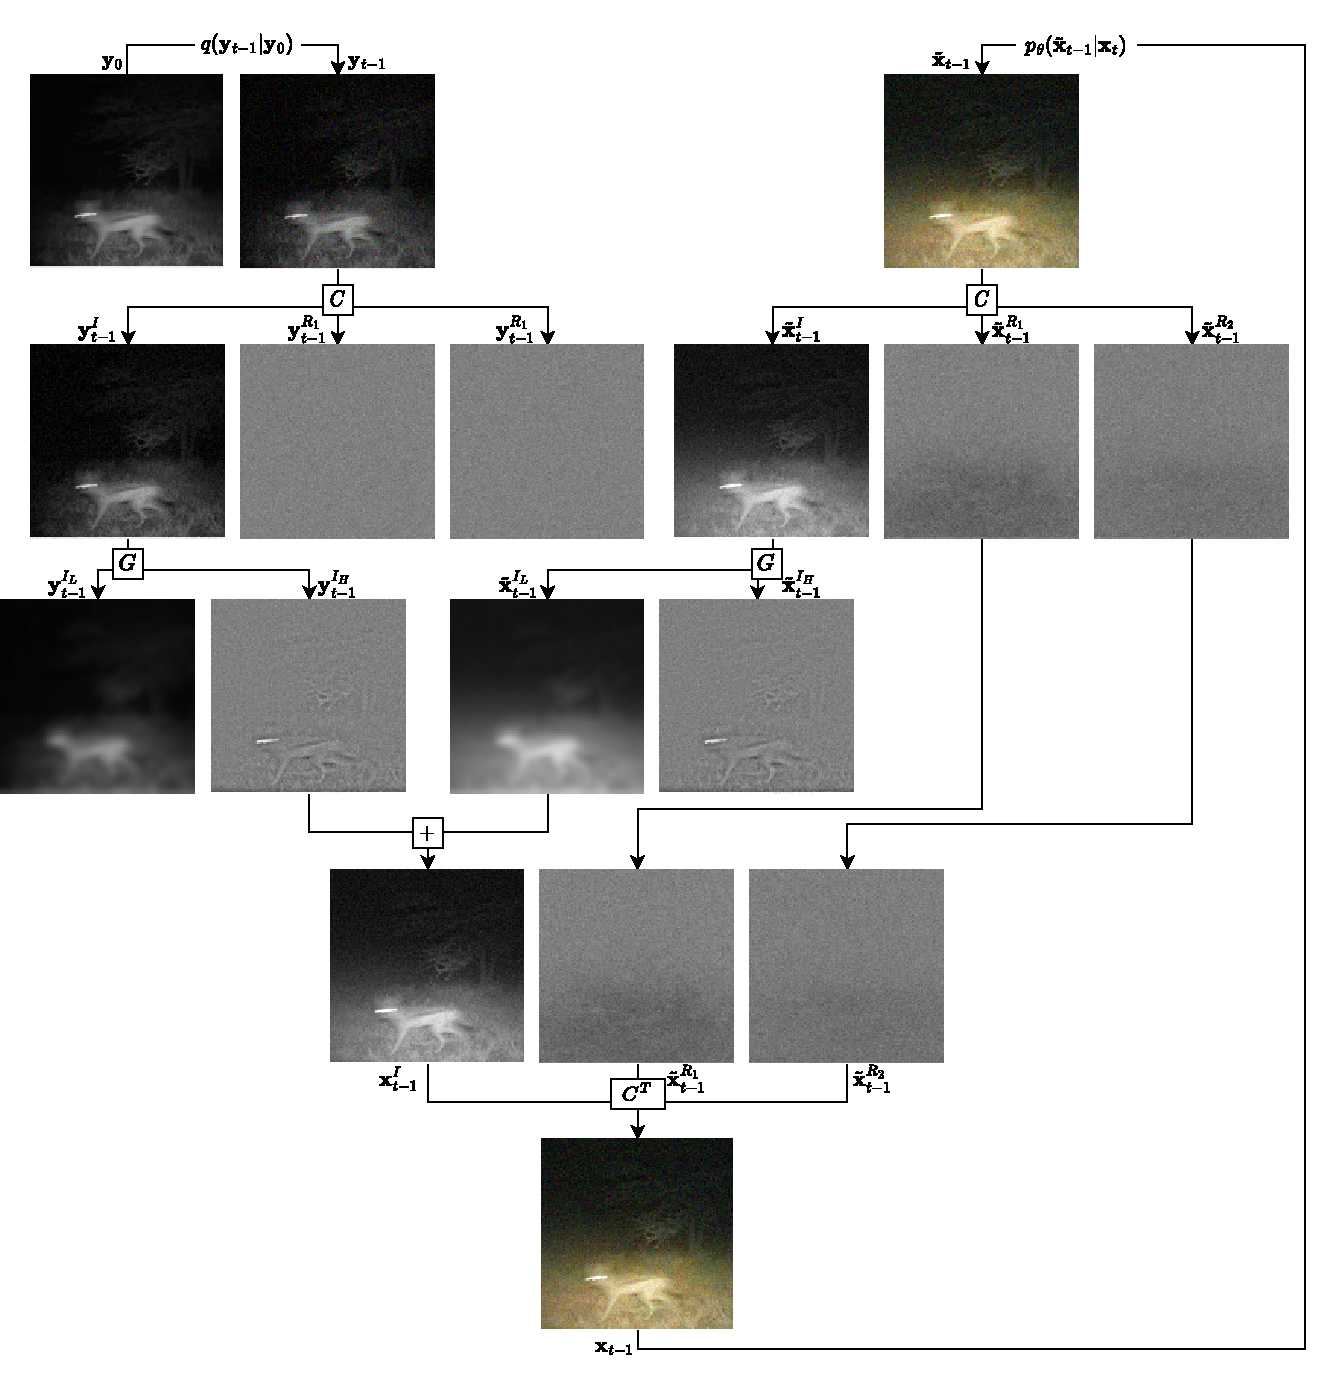
\includegraphics[width=\textwidth]{gfx/NIR-Colorization-Sampling.pdf}
   \caption{
      \textbf{Iteration Schema for Colorization using High-Frequency Intensity Replacement}.
      First approximate $\tilde{\x}_{t-1}$ and noised input image are $\y_{t-1}$ sampled with $p_\theta(\x_{t-1}|\x_t)$ and $q(\y_{t-1}|\y_0)$ respectively.
      Both are then decomposed into intensity and remaining dimensions. 
      Of both intensity dimensions $\y_{t-1}^I$ and $\tilde{\x}_{t-1}^I$ high- and low-frequency are obtained.  
      High-frequency intensities of the noised input image $\y_{t-1}^{I_H}$ are combined with low-frequency intensity of the approximate sample $\tilde{\x}_{t-1}^{I_H}$ to form the resulting intensity $\x_{t-1}^{I}$.
      Finally, the resulting intensity $\x_{t-1}^{I}$ is merged with color of the approximate sample $\tilde{\x}_{t-1}^R$ and transformed back into regular RGB domain, obtaining $\x_{t-1}$ (\autoref{alg:sampling-nir-colorization}).
      $C$ denotes decomposition function into intensity and remaining dimensions while $G$ denotes decomposition in low- and high-frequencies.
   }
   \label{fig:sampling-nir-colorization}
\end{figure}

\todo{Connection to \autoref{sec:conditional-sampling}}

\subsection{Energy-Guided Conditional Sampling}
\label{sec:energy-guided-sampling}
Based on the derivation in \autoref{sec:conditional-sampling}, \textcite{egsde} propose to guide the sampling using an energy-function.
Given an input image $\y_0$, we define $p_\theta(\y_0|\x_t)$ as \autoref{eqn:enery-definition}.

\begin{equation}
   \label{eqn:enery-definition}
   p_\theta(\y_0|\x_t) = \exp(\mathcal{E}(\x_t, \y_0, t))
\end{equation}

To guide the image generation using the diffusion network the energy function must be designed.

As further discussed in \autoref{sec:correction-guided-sampling},
we could now model the energy function either by comparing the intensities (\autoref{eqn:energy-intensities}) or by comparing the high frequencies of the intensities (\autoref{eqn:energy-high-freq-intensities}).
Here, the $\x^I_t$ and $\y^I_t$ denote the intensities of the sample image $\x_t$ and a noised NIR image $\y_t$ while $\x^{I_H}_t$ and $\y^{I_H}_t$  denote the high frequencies of the intensities respectively.

\begin{align}
   \mathcal{E}_I(\x_t, \y_0, t)     & = \mathbb{E}_{\y_t \sim p(\y_t | \y_0)}\left[|| \x^I_t - \y^I_t ||^2\right] \label{eqn:energy-intensities}                   \\
   \mathcal{E}_{I_H}(\x_t, \y_0, t) & = \mathbb{E}_{\y_t \sim p(\y_t | \y_0)}\left[|| \x^{I_H}_t - \y^{I_H}_t ||^2\right] \label{eqn:energy-high-freq-intensities}
\end{align}


\todo{Maybe extend this more, provide intuition}

\todo{Maybe visualize something here}